\section{File System Implementation}

\paragraph{Disk Structure}
\begin{itemize}
  \item \textbf{Partitions}: disk can be subdivided into partitions
  \item \textbf{Raw usage}: disks/partitions can be used raw (unformatted) or formatted with file system
  \item \textbf{Volume}: entry containing FS
  \begin{itemize}
    \item tracks that file system's info is in device directory or volume table of contents
  \end{itemize}
  \item \textbf{FS diversity}: there are general purpose and special purpose FS
\end{itemize}

\paragraph{File Systems --- Logical vs. Physical}
\begin{itemize}
  \item \textbf{Logical}: can consist of different physical file systems
  \item \textbf{Placement}: file system can be mounted at any place within another file system
  \item \textbf{Mounted local root}: bit in i-node of local root in mounted file system identifies this directory as mount point
\end{itemize}

\paragraph{File Systems --- Layers}
\begin{itemize}
  \item \textbf{Layer 5}: applications
  \item \textbf{Layer 4}: logical file system
  \item \textbf{Layer 3}: file-organization module
  \item \textbf{Layer 2}: basic file system
  \item \textbf{Layer 1}: I/O control
  \item \textbf{Layer 0}: devices
\end{itemize}

\paragraph{File Systems --- Virtual}
\begin{itemize}
  \item \textbf{Principle}: provide object-oriented way of implementing file systems
  \begin{itemize}
    \item same API used for different file system types
  \end{itemize}
\end{itemize}
\begin{figure}[h]\centering\label{VirtualFileSystem}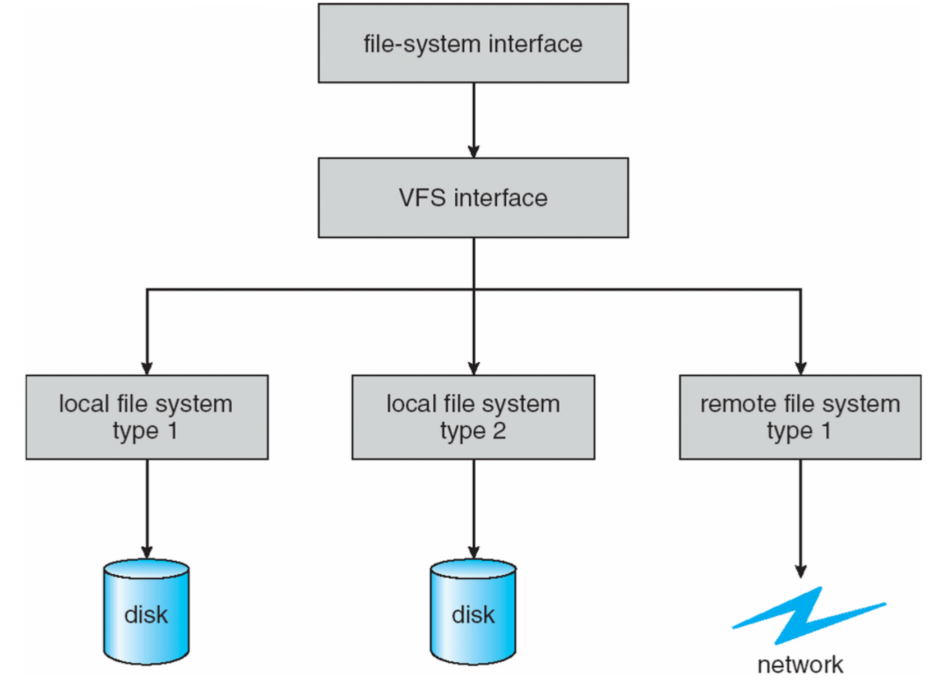
\includegraphics[width=0.33\textwidth]{VirtualFileSystem}\end{figure}

\paragraph{Files --- Implementation}
\begin{itemize}
  \item \textbf{Meta data} must be tracked:
  \begin{itemize}
    \item which logical block belongs to which file?
    \item block order?
    \item which blocks are free for next allocation?
  \end{itemize}
  \item \textbf{Block identification}: blocks on disk must be identified by FS (given logical region of file)
  \begin{itemize}
    \item[$ \to $] meta data needed in \emph{file allocation table}, \emph{directory} and \emph{inode}
  \end{itemize}
  \item \textbf{Block management}: creating/updating files might imply allocating new/modifying old disk blocks
\end{itemize}

\paragraph{Allocation --- Policies}
\begin{itemize}
  \item \textbf{Preallocation}:
  \begin{itemize}
    \item \emph{problem}: need to know maximum file size at creation time
    \item often difficult to reliably estimate maximum file size
    \item users tend to overestimate file size to avoid running out of space
  \end{itemize}
  \item \textbf{Dynamic allocation}: allocate in pieces as needed
\end{itemize}

\paragraph{Allocation --- Fragment size}
\begin{itemize}
  \item \textbf{Extremes}:
  \begin{itemize}
    \item fragment size = length of file
    \item fragment size = smallest disk block size (= sector size)
  \end{itemize}
  \item \textbf{Trade-offs}:
  \begin{itemize}
    \item \emph{contiguity}: speedup for sequential accesses
    \item \emph{small fragments}: larger tables needed to manage free storage and file access
    \item \emph{large fragments}: improve data transfer
    \item \emph{fixed-size fragments}: simplifies space reallocation
    \item \emph{variable-size fragments}: minimizes internal fragmentation, can lead to external fragmentation
  \end{itemize}
\end{itemize}

\paragraph{Allocation --- File space}
\begin{itemize}
  \item \textbf{Contiguous}
  \item \textbf{Chained}
  \item \textbf{Indexed}:
  \begin{itemize}
    \item fixed block fragments
    \item variable block fragments
  \end{itemize}
\end{itemize}
\begin{figure}[h]\centering\label{AllocationOverview}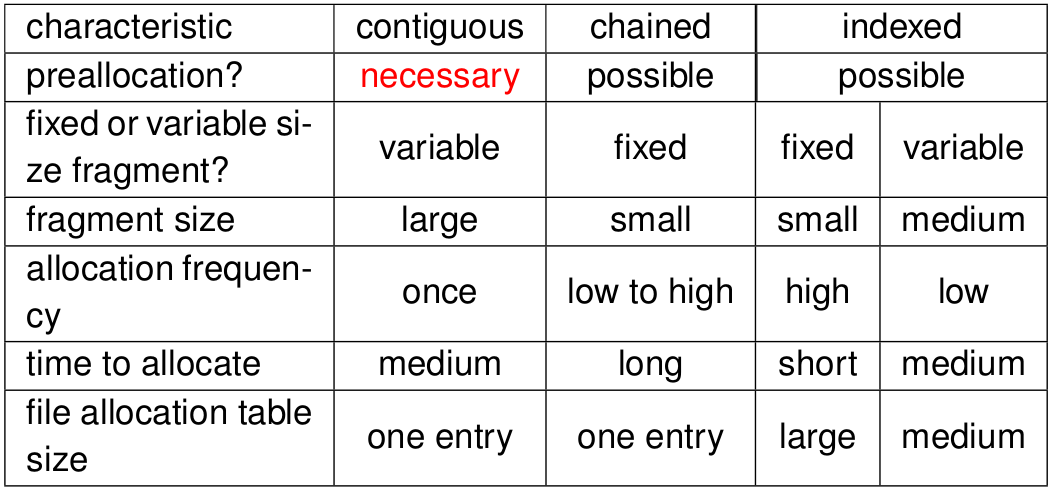
\includegraphics[width=0.33\textwidth]{AllocationOverview}\end{figure}

\paragraph{Allocation --- Contiguous}
\begin{itemize}
  \item \textbf{Principle}: array of $ n $ contiguous logical blocks reserved per file (to be created)
  \item \textbf{Periodic compaction}: overcome external fragmentation
\end{itemize}
\begin{figure}[h]\centering\label{AllocationContiguous}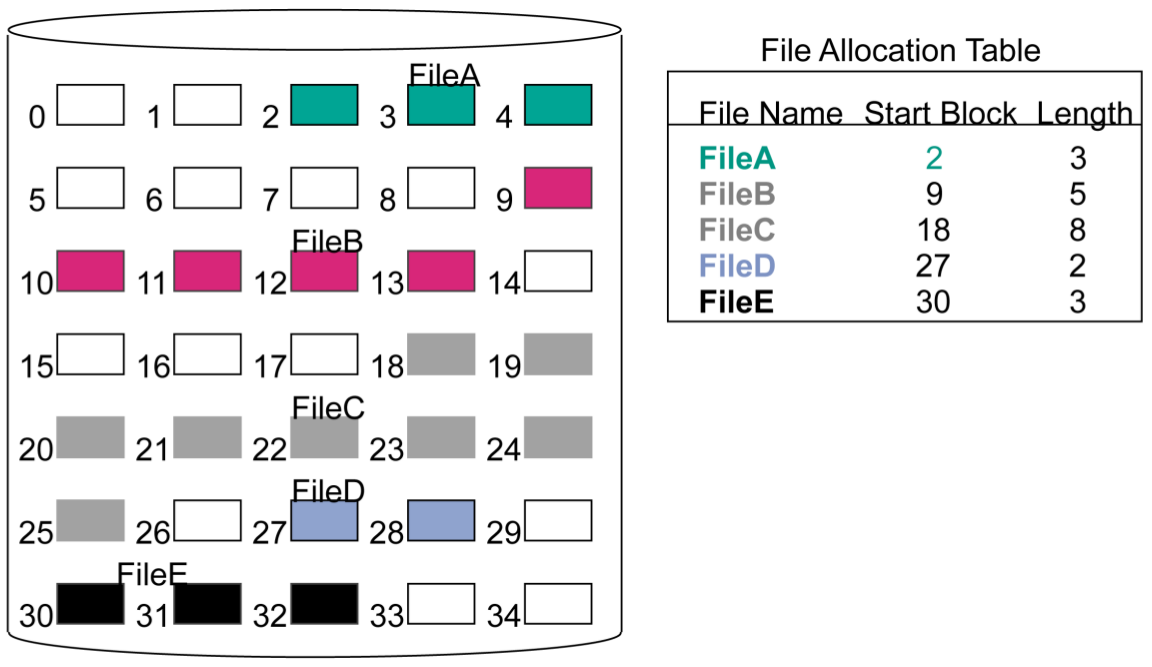
\includegraphics[width=0.33\textwidth]{AllocationContiguous}\end{figure}

\paragraph{Allocation --- Chained}
\begin{itemize}
  \item \textbf{Principle}: linked list of logical blocks per file
  \begin{itemize}
    \item FAT or directory contains address of first file block
    \item[$ \to $] \emph{no external fragmentation}: any free block can be added to chain
  \end{itemize}
\end{itemize}
\begin{figure}[h]\centering\label{AllocationChained}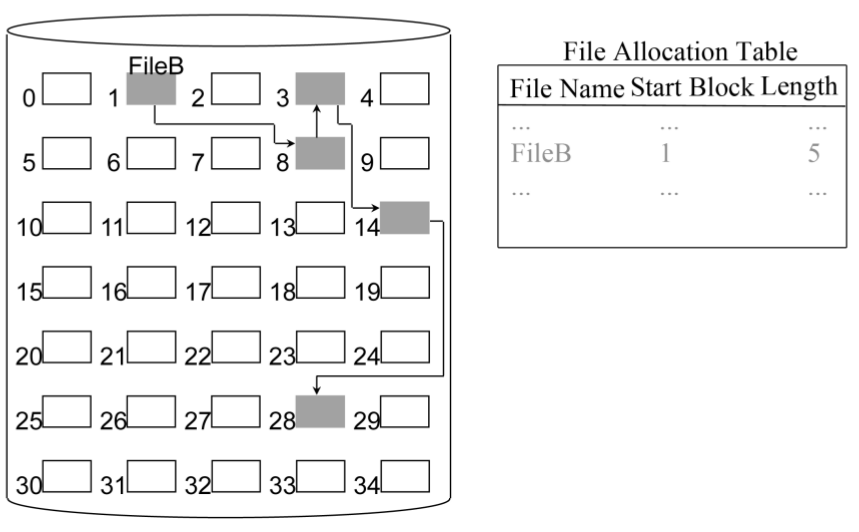
\includegraphics[width=0.33\textwidth]{AllocationChained}\end{figure}

\paragraph{Allocation --- Indexed}
\begin{itemize}
  \item \textbf{Principle}: FAT contains one-level index table per file
  \begin{itemize}
    \item \emph{generalization}: $ n $-level index table
    \item index has one entry for allocated file block
    \item FAT contains block number for index
  \end{itemize}
\end{itemize}
\begin{figure}[h]\centering\label{AllocationIndexed}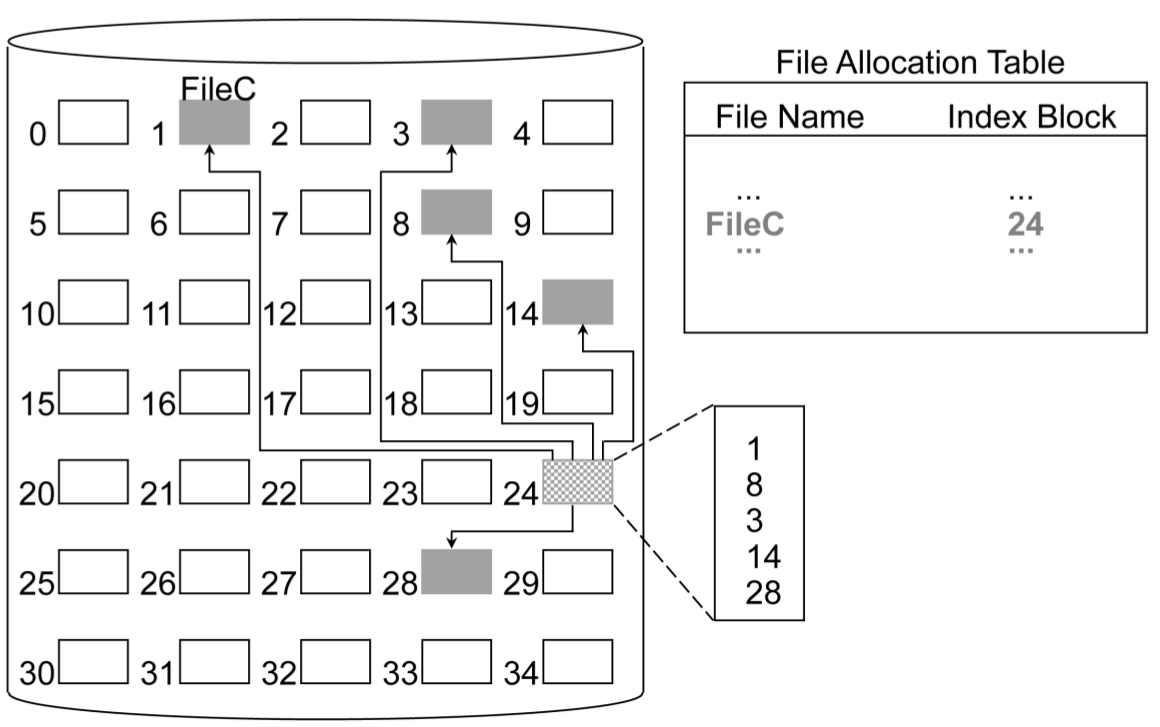
\includegraphics[width=0.33\textwidth]{AllocationIndexed}\end{figure}

\paragraph{Directories --- Implementation}
\begin{itemize}
  \item \textbf{Simple directory} (MS-DOS):
  \begin{itemize}
    \item fixed-size entries
    \item disk addresses + attributes in directory entry
  \end{itemize}
  \item \textbf{i-node reference directory} (UNIX):
  \begin{itemize}
    \item entry refers to i-node containing attributes
  \end{itemize}
\end{itemize}

\paragraph{Disk Blocks --- Buffering}
\begin{itemize}
  \item \textbf{Buffering}: disk blocks buffered in main memory
  \item \textbf{Access}: buffer access done via hash table
  \begin{itemize}
    \item blocks with same hash value are chained together
  \end{itemize}
  \item \textbf{Replacement}: LRU
  \item \textbf{Management}: free buffer is managed via doubly-linked list
\end{itemize}

\paragraph{File Systems --- Journaling}
\begin{itemize}
  \item \textbf{Principle}: record each update to file system as \emph{transaction}
  \begin{itemize}
    \item written to log
  \end{itemize}
  \item \textbf{Committed} transaction = written to log
  \begin{itemize}
    \item[$ \to $] \emph{problem}: file system may not yet be updated
  \end{itemize}
  \item \textbf{Writing} transactions from log to FS is asynchronous
  \item \textbf{Modifying} FS $ \to $ transaction removed from log
  \item \textbf{Crash} of file system $ \to $ remaining transactions in log must still be performed
\end{itemize}

\paragraph{File Systems --- Log-structured}
\begin{itemize}
  \item \textbf{Principle}: use disk as circular buffer
  \begin{itemize}
    \item write all updated (including i-nodes, meta data and data) to end of log
  \end{itemize}
  \item \textbf{Buffering}: all writes initially buffered in memory
  \item \textbf{Writing}: periodically write within 1 segment (1 MB)
  \item \textbf{Opening}: locate i-node, find blocks
  \item \textbf{Clearing}: clear all data from other end, no longer used
\end{itemize}